% Created by tikzDevice version 0.10.1 on 2017-11-19 19:18:31
% !TEX encoding = UTF-8 Unicode
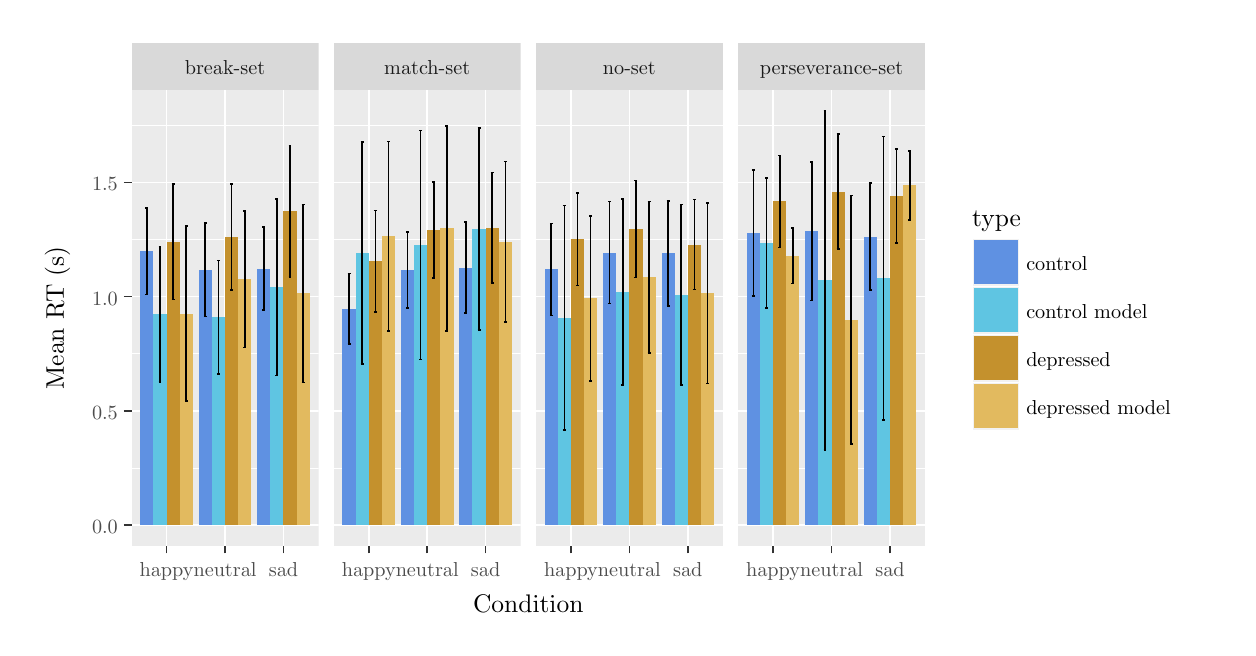
\begin{tikzpicture}[x=1pt,y=1pt]
\definecolor{fillColor}{RGB}{255,255,255}
\path[use as bounding box,fill=fillColor,fill opacity=0.00] (0,0) rectangle (433.62,216.81);
\begin{scope}
\path[clip] (  0.00,  0.00) rectangle (433.62,216.81);
\definecolor{drawColor}{RGB}{255,255,255}
\definecolor{fillColor}{RGB}{255,255,255}

\path[draw=drawColor,line width= 0.6pt,line join=round,line cap=round,fill=fillColor] (  0.00,  0.00) rectangle (433.62,216.81);
\end{scope}
\begin{scope}
\path[clip] ( 37.53, 29.59) rectangle (105.09,194.25);
\definecolor{fillColor}{gray}{0.92}

\path[fill=fillColor] ( 37.53, 29.59) rectangle (105.09,194.25);
\definecolor{drawColor}{RGB}{255,255,255}

\path[draw=drawColor,line width= 0.3pt,line join=round] ( 37.53, 57.71) --
	(105.09, 57.71);

\path[draw=drawColor,line width= 0.3pt,line join=round] ( 37.53, 98.97) --
	(105.09, 98.97);

\path[draw=drawColor,line width= 0.3pt,line join=round] ( 37.53,140.24) --
	(105.09,140.24);

\path[draw=drawColor,line width= 0.3pt,line join=round] ( 37.53,181.51) --
	(105.09,181.51);

\path[draw=drawColor,line width= 0.6pt,line join=round] ( 37.53, 37.07) --
	(105.09, 37.07);

\path[draw=drawColor,line width= 0.6pt,line join=round] ( 37.53, 78.34) --
	(105.09, 78.34);

\path[draw=drawColor,line width= 0.6pt,line join=round] ( 37.53,119.61) --
	(105.09,119.61);

\path[draw=drawColor,line width= 0.6pt,line join=round] ( 37.53,160.87) --
	(105.09,160.87);

\path[draw=drawColor,line width= 0.6pt,line join=round] ( 50.20, 29.59) --
	( 50.20,194.25);

\path[draw=drawColor,line width= 0.6pt,line join=round] ( 71.31, 29.59) --
	( 71.31,194.25);

\path[draw=drawColor,line width= 0.6pt,line join=round] ( 92.42, 29.59) --
	( 92.42,194.25);
\definecolor{fillColor}{RGB}{226,186,95}

\path[fill=fillColor] ( 54.95, 37.07) rectangle ( 59.70,113.43);
\definecolor{fillColor}{RGB}{196,145,45}

\path[fill=fillColor] ( 50.20, 37.07) rectangle ( 54.95,139.50);
\definecolor{fillColor}{RGB}{95,197,226}

\path[fill=fillColor] ( 45.45, 37.07) rectangle ( 50.20,113.21);
\definecolor{fillColor}{RGB}{95,145,226}

\path[fill=fillColor] ( 40.70, 37.07) rectangle ( 45.45,136.03);
\definecolor{fillColor}{RGB}{226,186,95}

\path[fill=fillColor] ( 76.06, 37.07) rectangle ( 80.81,125.86);
\definecolor{fillColor}{RGB}{196,145,45}

\path[fill=fillColor] ( 71.31, 37.07) rectangle ( 76.06,141.15);
\definecolor{fillColor}{RGB}{95,197,226}

\path[fill=fillColor] ( 66.56, 37.07) rectangle ( 71.31,112.21);
\definecolor{fillColor}{RGB}{95,145,226}

\path[fill=fillColor] ( 61.81, 37.07) rectangle ( 66.56,129.35);
\definecolor{fillColor}{RGB}{226,186,95}

\path[fill=fillColor] ( 97.17, 37.07) rectangle (101.92,120.81);
\definecolor{fillColor}{RGB}{196,145,45}

\path[fill=fillColor] ( 92.42, 37.07) rectangle ( 97.17,150.47);
\definecolor{fillColor}{RGB}{95,197,226}

\path[fill=fillColor] ( 87.67, 37.07) rectangle ( 92.42,122.95);
\definecolor{fillColor}{RGB}{95,145,226}

\path[fill=fillColor] ( 82.92, 37.07) rectangle ( 87.67,129.76);
\definecolor{drawColor}{RGB}{0,0,0}

\path[draw=drawColor,line width= 0.6pt,line join=round] ( 56.80,145.07) --
	( 57.85,145.07);

\path[draw=drawColor,line width= 0.6pt,line join=round] ( 57.32,145.07) --
	( 57.32, 81.80);

\path[draw=drawColor,line width= 0.6pt,line join=round] ( 56.80, 81.80) --
	( 57.85, 81.80);

\path[draw=drawColor,line width= 0.6pt,line join=round] ( 52.05,160.38) --
	( 53.10,160.38);

\path[draw=drawColor,line width= 0.6pt,line join=round] ( 52.57,160.38) --
	( 52.57,118.62);

\path[draw=drawColor,line width= 0.6pt,line join=round] ( 52.05,118.62) --
	( 53.10,118.62);

\path[draw=drawColor,line width= 0.6pt,line join=round] ( 47.30,137.76) --
	( 48.35,137.76);

\path[draw=drawColor,line width= 0.6pt,line join=round] ( 47.82,137.76) --
	( 47.82, 88.67);

\path[draw=drawColor,line width= 0.6pt,line join=round] ( 47.30, 88.67) --
	( 48.35, 88.67);

\path[draw=drawColor,line width= 0.6pt,line join=round] ( 42.55,151.63) --
	( 43.60,151.63);

\path[draw=drawColor,line width= 0.6pt,line join=round] ( 43.07,151.63) --
	( 43.07,120.43);

\path[draw=drawColor,line width= 0.6pt,line join=round] ( 42.55,120.43) --
	( 43.60,120.43);

\path[draw=drawColor,line width= 0.6pt,line join=round] ( 77.91,150.50) --
	( 78.96,150.50);

\path[draw=drawColor,line width= 0.6pt,line join=round] ( 78.44,150.50) --
	( 78.44,101.21);

\path[draw=drawColor,line width= 0.6pt,line join=round] ( 77.91,101.21) --
	( 78.96,101.21);

\path[draw=drawColor,line width= 0.6pt,line join=round] ( 73.16,160.30) --
	( 74.21,160.30);

\path[draw=drawColor,line width= 0.6pt,line join=round] ( 73.69,160.30) --
	( 73.69,122.00);

\path[draw=drawColor,line width= 0.6pt,line join=round] ( 73.16,122.00) --
	( 74.21,122.00);

\path[draw=drawColor,line width= 0.6pt,line join=round] ( 68.41,132.65) --
	( 69.46,132.65);

\path[draw=drawColor,line width= 0.6pt,line join=round] ( 68.94,132.65) --
	( 68.94, 91.78);

\path[draw=drawColor,line width= 0.6pt,line join=round] ( 68.41, 91.78) --
	( 69.46, 91.78);

\path[draw=drawColor,line width= 0.6pt,line join=round] ( 63.66,146.27) --
	( 64.71,146.27);

\path[draw=drawColor,line width= 0.6pt,line join=round] ( 64.19,146.27) --
	( 64.19,112.43);

\path[draw=drawColor,line width= 0.6pt,line join=round] ( 63.66,112.43) --
	( 64.71,112.43);

\path[draw=drawColor,line width= 0.6pt,line join=round] ( 99.02,152.97) --
	(100.07,152.97);

\path[draw=drawColor,line width= 0.6pt,line join=round] ( 99.55,152.97) --
	( 99.55, 88.65);

\path[draw=drawColor,line width= 0.6pt,line join=round] ( 99.02, 88.65) --
	(100.07, 88.65);

\path[draw=drawColor,line width= 0.6pt,line join=round] ( 94.27,174.24) --
	( 95.32,174.24);

\path[draw=drawColor,line width= 0.6pt,line join=round] ( 94.80,174.24) --
	( 94.80,126.70);

\path[draw=drawColor,line width= 0.6pt,line join=round] ( 94.27,126.70) --
	( 95.32,126.70);

\path[draw=drawColor,line width= 0.6pt,line join=round] ( 89.52,154.78) --
	( 90.57,154.78);

\path[draw=drawColor,line width= 0.6pt,line join=round] ( 90.05,154.78) --
	( 90.05, 91.13);

\path[draw=drawColor,line width= 0.6pt,line join=round] ( 89.52, 91.13) --
	( 90.57, 91.13);

\path[draw=drawColor,line width= 0.6pt,line join=round] ( 84.77,144.70) --
	( 85.82,144.70);

\path[draw=drawColor,line width= 0.6pt,line join=round] ( 85.30,144.70) --
	( 85.30,114.82);

\path[draw=drawColor,line width= 0.6pt,line join=round] ( 84.77,114.82) --
	( 85.82,114.82);
\end{scope}
\begin{scope}
\path[clip] (110.59, 29.59) rectangle (178.14,194.25);
\definecolor{fillColor}{gray}{0.92}

\path[fill=fillColor] (110.59, 29.59) rectangle (178.14,194.25);
\definecolor{drawColor}{RGB}{255,255,255}

\path[draw=drawColor,line width= 0.3pt,line join=round] (110.59, 57.71) --
	(178.14, 57.71);

\path[draw=drawColor,line width= 0.3pt,line join=round] (110.59, 98.97) --
	(178.14, 98.97);

\path[draw=drawColor,line width= 0.3pt,line join=round] (110.59,140.24) --
	(178.14,140.24);

\path[draw=drawColor,line width= 0.3pt,line join=round] (110.59,181.51) --
	(178.14,181.51);

\path[draw=drawColor,line width= 0.6pt,line join=round] (110.59, 37.07) --
	(178.14, 37.07);

\path[draw=drawColor,line width= 0.6pt,line join=round] (110.59, 78.34) --
	(178.14, 78.34);

\path[draw=drawColor,line width= 0.6pt,line join=round] (110.59,119.61) --
	(178.14,119.61);

\path[draw=drawColor,line width= 0.6pt,line join=round] (110.59,160.87) --
	(178.14,160.87);

\path[draw=drawColor,line width= 0.6pt,line join=round] (123.25, 29.59) --
	(123.25,194.25);

\path[draw=drawColor,line width= 0.6pt,line join=round] (144.37, 29.59) --
	(144.37,194.25);

\path[draw=drawColor,line width= 0.6pt,line join=round] (165.48, 29.59) --
	(165.48,194.25);
\definecolor{fillColor}{RGB}{226,186,95}

\path[fill=fillColor] (128.00, 37.07) rectangle (132.75,141.44);
\definecolor{fillColor}{RGB}{196,145,45}

\path[fill=fillColor] (123.25, 37.07) rectangle (128.00,132.48);
\definecolor{fillColor}{RGB}{95,197,226}

\path[fill=fillColor] (118.50, 37.07) rectangle (123.25,135.40);
\definecolor{fillColor}{RGB}{95,145,226}

\path[fill=fillColor] (113.75, 37.07) rectangle (118.50,115.31);
\definecolor{fillColor}{RGB}{226,186,95}

\path[fill=fillColor] (149.12, 37.07) rectangle (153.87,144.27);
\definecolor{fillColor}{RGB}{196,145,45}

\path[fill=fillColor] (144.37, 37.07) rectangle (149.12,143.71);
\definecolor{fillColor}{RGB}{95,197,226}

\path[fill=fillColor] (139.62, 37.07) rectangle (144.37,138.25);
\definecolor{fillColor}{RGB}{95,145,226}

\path[fill=fillColor] (134.87, 37.07) rectangle (139.62,129.26);
\definecolor{fillColor}{RGB}{226,186,95}

\path[fill=fillColor] (170.23, 37.07) rectangle (174.98,139.46);
\definecolor{fillColor}{RGB}{196,145,45}

\path[fill=fillColor] (165.48, 37.07) rectangle (170.23,144.53);
\definecolor{fillColor}{RGB}{95,197,226}

\path[fill=fillColor] (160.73, 37.07) rectangle (165.48,144.13);
\definecolor{fillColor}{RGB}{95,145,226}

\path[fill=fillColor] (155.98, 37.07) rectangle (160.73,130.09);
\definecolor{drawColor}{RGB}{0,0,0}

\path[draw=drawColor,line width= 0.6pt,line join=round] (129.85,175.62) --
	(130.91,175.62);

\path[draw=drawColor,line width= 0.6pt,line join=round] (130.38,175.62) --
	(130.38,107.26);

\path[draw=drawColor,line width= 0.6pt,line join=round] (129.85,107.26) --
	(130.91,107.26);

\path[draw=drawColor,line width= 0.6pt,line join=round] (125.10,150.80) --
	(126.16,150.80);

\path[draw=drawColor,line width= 0.6pt,line join=round] (125.63,150.80) --
	(125.63,114.16);

\path[draw=drawColor,line width= 0.6pt,line join=round] (125.10,114.16) --
	(126.16,114.16);

\path[draw=drawColor,line width= 0.6pt,line join=round] (120.35,175.46) --
	(121.41,175.46);

\path[draw=drawColor,line width= 0.6pt,line join=round] (120.88,175.46) --
	(120.88, 95.34);

\path[draw=drawColor,line width= 0.6pt,line join=round] (120.35, 95.34) --
	(121.41, 95.34);

\path[draw=drawColor,line width= 0.6pt,line join=round] (115.60,128.03) --
	(116.66,128.03);

\path[draw=drawColor,line width= 0.6pt,line join=round] (116.13,128.03) --
	(116.13,102.60);

\path[draw=drawColor,line width= 0.6pt,line join=round] (115.60,102.60) --
	(116.66,102.60);

\path[draw=drawColor,line width= 0.6pt,line join=round] (150.96,181.24) --
	(152.02,181.24);

\path[draw=drawColor,line width= 0.6pt,line join=round] (151.49,181.24) --
	(151.49,107.29);

\path[draw=drawColor,line width= 0.6pt,line join=round] (150.96,107.29) --
	(152.02,107.29);

\path[draw=drawColor,line width= 0.6pt,line join=round] (146.21,160.96) --
	(147.27,160.96);

\path[draw=drawColor,line width= 0.6pt,line join=round] (146.74,160.96) --
	(146.74,126.46);

\path[draw=drawColor,line width= 0.6pt,line join=round] (146.21,126.46) --
	(147.27,126.46);

\path[draw=drawColor,line width= 0.6pt,line join=round] (141.46,179.59) --
	(142.52,179.59);

\path[draw=drawColor,line width= 0.6pt,line join=round] (141.99,179.59) --
	(141.99, 96.90);

\path[draw=drawColor,line width= 0.6pt,line join=round] (141.46, 96.90) --
	(142.52, 96.90);

\path[draw=drawColor,line width= 0.6pt,line join=round] (136.71,143.05) --
	(137.77,143.05);

\path[draw=drawColor,line width= 0.6pt,line join=round] (137.24,143.05) --
	(137.24,115.48);

\path[draw=drawColor,line width= 0.6pt,line join=round] (136.71,115.48) --
	(137.77,115.48);

\path[draw=drawColor,line width= 0.6pt,line join=round] (172.07,168.42) --
	(173.13,168.42);

\path[draw=drawColor,line width= 0.6pt,line join=round] (172.60,168.42) --
	(172.60,110.51);

\path[draw=drawColor,line width= 0.6pt,line join=round] (172.07,110.51) --
	(173.13,110.51);

\path[draw=drawColor,line width= 0.6pt,line join=round] (167.32,164.42) --
	(168.38,164.42);

\path[draw=drawColor,line width= 0.6pt,line join=round] (167.85,164.42) --
	(167.85,124.64);

\path[draw=drawColor,line width= 0.6pt,line join=round] (167.32,124.64) --
	(168.38,124.64);

\path[draw=drawColor,line width= 0.6pt,line join=round] (162.57,180.65) --
	(163.63,180.65);

\path[draw=drawColor,line width= 0.6pt,line join=round] (163.10,180.65) --
	(163.10,107.61);

\path[draw=drawColor,line width= 0.6pt,line join=round] (162.57,107.61) --
	(163.63,107.61);

\path[draw=drawColor,line width= 0.6pt,line join=round] (157.82,146.51) --
	(158.88,146.51);

\path[draw=drawColor,line width= 0.6pt,line join=round] (158.35,146.51) --
	(158.35,113.66);

\path[draw=drawColor,line width= 0.6pt,line join=round] (157.82,113.66) --
	(158.88,113.66);
\end{scope}
\begin{scope}
\path[clip] (183.64, 29.59) rectangle (251.20,194.25);
\definecolor{fillColor}{gray}{0.92}

\path[fill=fillColor] (183.64, 29.59) rectangle (251.20,194.25);
\definecolor{drawColor}{RGB}{255,255,255}

\path[draw=drawColor,line width= 0.3pt,line join=round] (183.64, 57.71) --
	(251.20, 57.71);

\path[draw=drawColor,line width= 0.3pt,line join=round] (183.64, 98.97) --
	(251.20, 98.97);

\path[draw=drawColor,line width= 0.3pt,line join=round] (183.64,140.24) --
	(251.20,140.24);

\path[draw=drawColor,line width= 0.3pt,line join=round] (183.64,181.51) --
	(251.20,181.51);

\path[draw=drawColor,line width= 0.6pt,line join=round] (183.64, 37.07) --
	(251.20, 37.07);

\path[draw=drawColor,line width= 0.6pt,line join=round] (183.64, 78.34) --
	(251.20, 78.34);

\path[draw=drawColor,line width= 0.6pt,line join=round] (183.64,119.61) --
	(251.20,119.61);

\path[draw=drawColor,line width= 0.6pt,line join=round] (183.64,160.87) --
	(251.20,160.87);

\path[draw=drawColor,line width= 0.6pt,line join=round] (196.31, 29.59) --
	(196.31,194.25);

\path[draw=drawColor,line width= 0.6pt,line join=round] (217.42, 29.59) --
	(217.42,194.25);

\path[draw=drawColor,line width= 0.6pt,line join=round] (238.53, 29.59) --
	(238.53,194.25);
\definecolor{fillColor}{RGB}{226,186,95}

\path[fill=fillColor] (201.06, 37.07) rectangle (205.81,118.96);
\definecolor{fillColor}{RGB}{196,145,45}

\path[fill=fillColor] (196.31, 37.07) rectangle (201.06,140.32);
\definecolor{fillColor}{RGB}{95,197,226}

\path[fill=fillColor] (191.56, 37.07) rectangle (196.31,111.96);
\definecolor{fillColor}{RGB}{95,145,226}

\path[fill=fillColor] (186.81, 37.07) rectangle (191.56,129.43);
\definecolor{fillColor}{RGB}{226,186,95}

\path[fill=fillColor] (222.17, 37.07) rectangle (226.92,126.70);
\definecolor{fillColor}{RGB}{196,145,45}

\path[fill=fillColor] (217.42, 37.07) rectangle (222.17,144.04);
\definecolor{fillColor}{RGB}{95,197,226}

\path[fill=fillColor] (212.67, 37.07) rectangle (217.42,121.30);
\definecolor{fillColor}{RGB}{95,145,226}

\path[fill=fillColor] (207.92, 37.07) rectangle (212.67,135.54);
\definecolor{fillColor}{RGB}{226,186,95}

\path[fill=fillColor] (243.28, 37.07) rectangle (248.03,120.88);
\definecolor{fillColor}{RGB}{196,145,45}

\path[fill=fillColor] (238.53, 37.07) rectangle (243.28,138.42);
\definecolor{fillColor}{RGB}{95,197,226}

\path[fill=fillColor] (233.78, 37.07) rectangle (238.53,120.28);
\definecolor{fillColor}{RGB}{95,145,226}

\path[fill=fillColor] (229.03, 37.07) rectangle (233.78,135.29);
\definecolor{drawColor}{RGB}{0,0,0}

\path[draw=drawColor,line width= 0.6pt,line join=round] (202.91,148.87) --
	(203.96,148.87);

\path[draw=drawColor,line width= 0.6pt,line join=round] (203.43,148.87) --
	(203.43, 89.04);

\path[draw=drawColor,line width= 0.6pt,line join=round] (202.91, 89.04) --
	(203.96, 89.04);

\path[draw=drawColor,line width= 0.6pt,line join=round] (198.16,157.00) --
	(199.21,157.00);

\path[draw=drawColor,line width= 0.6pt,line join=round] (198.68,157.00) --
	(198.68,123.65);

\path[draw=drawColor,line width= 0.6pt,line join=round] (198.16,123.65) --
	(199.21,123.65);

\path[draw=drawColor,line width= 0.6pt,line join=round] (193.41,152.51) --
	(194.46,152.51);

\path[draw=drawColor,line width= 0.6pt,line join=round] (193.93,152.51) --
	(193.93, 71.41);

\path[draw=drawColor,line width= 0.6pt,line join=round] (193.41, 71.41) --
	(194.46, 71.41);

\path[draw=drawColor,line width= 0.6pt,line join=round] (188.66,146.02) --
	(189.71,146.02);

\path[draw=drawColor,line width= 0.6pt,line join=round] (189.18,146.02) --
	(189.18,112.84);

\path[draw=drawColor,line width= 0.6pt,line join=round] (188.66,112.84) --
	(189.71,112.84);

\path[draw=drawColor,line width= 0.6pt,line join=round] (224.02,154.03) --
	(225.07,154.03);

\path[draw=drawColor,line width= 0.6pt,line join=round] (224.55,154.03) --
	(224.55, 99.37);

\path[draw=drawColor,line width= 0.6pt,line join=round] (224.02, 99.37) --
	(225.07, 99.37);

\path[draw=drawColor,line width= 0.6pt,line join=round] (219.27,161.53) --
	(220.32,161.53);

\path[draw=drawColor,line width= 0.6pt,line join=round] (219.80,161.53) --
	(219.80,126.54);

\path[draw=drawColor,line width= 0.6pt,line join=round] (219.27,126.54) --
	(220.32,126.54);

\path[draw=drawColor,line width= 0.6pt,line join=round] (214.52,154.95) --
	(215.57,154.95);

\path[draw=drawColor,line width= 0.6pt,line join=round] (215.05,154.95) --
	(215.05, 87.64);

\path[draw=drawColor,line width= 0.6pt,line join=round] (214.52, 87.64) --
	(215.57, 87.64);

\path[draw=drawColor,line width= 0.6pt,line join=round] (209.77,153.94) --
	(210.82,153.94);

\path[draw=drawColor,line width= 0.6pt,line join=round] (210.30,153.94) --
	(210.30,117.13);

\path[draw=drawColor,line width= 0.6pt,line join=round] (209.77,117.13) --
	(210.82,117.13);

\path[draw=drawColor,line width= 0.6pt,line join=round] (245.13,153.54) --
	(246.18,153.54);

\path[draw=drawColor,line width= 0.6pt,line join=round] (245.66,153.54) --
	(245.66, 88.22);

\path[draw=drawColor,line width= 0.6pt,line join=round] (245.13, 88.22) --
	(246.18, 88.22);

\path[draw=drawColor,line width= 0.6pt,line join=round] (240.38,154.68) --
	(241.43,154.68);

\path[draw=drawColor,line width= 0.6pt,line join=round] (240.91,154.68) --
	(240.91,122.17);

\path[draw=drawColor,line width= 0.6pt,line join=round] (240.38,122.17) --
	(241.43,122.17);

\path[draw=drawColor,line width= 0.6pt,line join=round] (235.63,152.90) --
	(236.68,152.90);

\path[draw=drawColor,line width= 0.6pt,line join=round] (236.16,152.90) --
	(236.16, 87.67);

\path[draw=drawColor,line width= 0.6pt,line join=round] (235.63, 87.67) --
	(236.68, 87.67);

\path[draw=drawColor,line width= 0.6pt,line join=round] (230.88,154.27) --
	(231.93,154.27);

\path[draw=drawColor,line width= 0.6pt,line join=round] (231.41,154.27) --
	(231.41,116.31);

\path[draw=drawColor,line width= 0.6pt,line join=round] (230.88,116.31) --
	(231.93,116.31);
\end{scope}
\begin{scope}
\path[clip] (256.70, 29.59) rectangle (324.25,194.25);
\definecolor{fillColor}{gray}{0.92}

\path[fill=fillColor] (256.70, 29.59) rectangle (324.25,194.25);
\definecolor{drawColor}{RGB}{255,255,255}

\path[draw=drawColor,line width= 0.3pt,line join=round] (256.70, 57.71) --
	(324.25, 57.71);

\path[draw=drawColor,line width= 0.3pt,line join=round] (256.70, 98.97) --
	(324.25, 98.97);

\path[draw=drawColor,line width= 0.3pt,line join=round] (256.70,140.24) --
	(324.25,140.24);

\path[draw=drawColor,line width= 0.3pt,line join=round] (256.70,181.51) --
	(324.25,181.51);

\path[draw=drawColor,line width= 0.6pt,line join=round] (256.70, 37.07) --
	(324.25, 37.07);

\path[draw=drawColor,line width= 0.6pt,line join=round] (256.70, 78.34) --
	(324.25, 78.34);

\path[draw=drawColor,line width= 0.6pt,line join=round] (256.70,119.61) --
	(324.25,119.61);

\path[draw=drawColor,line width= 0.6pt,line join=round] (256.70,160.87) --
	(324.25,160.87);

\path[draw=drawColor,line width= 0.6pt,line join=round] (269.36, 29.59) --
	(269.36,194.25);

\path[draw=drawColor,line width= 0.6pt,line join=round] (290.48, 29.59) --
	(290.48,194.25);

\path[draw=drawColor,line width= 0.6pt,line join=round] (311.59, 29.59) --
	(311.59,194.25);
\definecolor{fillColor}{RGB}{226,186,95}

\path[fill=fillColor] (274.11, 37.07) rectangle (278.86,134.37);
\definecolor{fillColor}{RGB}{196,145,45}

\path[fill=fillColor] (269.36, 37.07) rectangle (274.11,154.02);
\definecolor{fillColor}{RGB}{95,197,226}

\path[fill=fillColor] (264.61, 37.07) rectangle (269.36,139.01);
\definecolor{fillColor}{RGB}{95,145,226}

\path[fill=fillColor] (259.86, 37.07) rectangle (264.61,142.55);
\definecolor{fillColor}{RGB}{226,186,95}

\path[fill=fillColor] (295.23, 37.07) rectangle (299.98,111.24);
\definecolor{fillColor}{RGB}{196,145,45}

\path[fill=fillColor] (290.48, 37.07) rectangle (295.23,157.57);
\definecolor{fillColor}{RGB}{95,197,226}

\path[fill=fillColor] (285.73, 37.07) rectangle (290.48,125.45);
\definecolor{fillColor}{RGB}{95,145,226}

\path[fill=fillColor] (280.98, 37.07) rectangle (285.73,143.21);
\definecolor{fillColor}{RGB}{226,186,95}

\path[fill=fillColor] (316.34, 37.07) rectangle (321.09,159.81);
\definecolor{fillColor}{RGB}{196,145,45}

\path[fill=fillColor] (311.59, 37.07) rectangle (316.34,156.00);
\definecolor{fillColor}{RGB}{95,197,226}

\path[fill=fillColor] (306.84, 37.07) rectangle (311.59,126.31);
\definecolor{fillColor}{RGB}{95,145,226}

\path[fill=fillColor] (302.09, 37.07) rectangle (306.84,141.31);
\definecolor{drawColor}{RGB}{0,0,0}

\path[draw=drawColor,line width= 0.6pt,line join=round] (275.96,144.36) --
	(277.02,144.36);

\path[draw=drawColor,line width= 0.6pt,line join=round] (276.49,144.36) --
	(276.49,124.37);

\path[draw=drawColor,line width= 0.6pt,line join=round] (275.96,124.37) --
	(277.02,124.37);

\path[draw=drawColor,line width= 0.6pt,line join=round] (271.21,170.61) --
	(272.27,170.61);

\path[draw=drawColor,line width= 0.6pt,line join=round] (271.74,170.61) --
	(271.74,137.43);

\path[draw=drawColor,line width= 0.6pt,line join=round] (271.21,137.43) --
	(272.27,137.43);

\path[draw=drawColor,line width= 0.6pt,line join=round] (266.46,162.42) --
	(267.52,162.42);

\path[draw=drawColor,line width= 0.6pt,line join=round] (266.99,162.42) --
	(266.99,115.60);

\path[draw=drawColor,line width= 0.6pt,line join=round] (266.46,115.60) --
	(267.52,115.60);

\path[draw=drawColor,line width= 0.6pt,line join=round] (261.71,165.33) --
	(262.77,165.33);

\path[draw=drawColor,line width= 0.6pt,line join=round] (262.24,165.33) --
	(262.24,119.77);

\path[draw=drawColor,line width= 0.6pt,line join=round] (261.71,119.77) --
	(262.77,119.77);

\path[draw=drawColor,line width= 0.6pt,line join=round] (297.07,156.12) --
	(298.13,156.12);

\path[draw=drawColor,line width= 0.6pt,line join=round] (297.60,156.12) --
	(297.60, 66.36);

\path[draw=drawColor,line width= 0.6pt,line join=round] (297.07, 66.36) --
	(298.13, 66.36);

\path[draw=drawColor,line width= 0.6pt,line join=round] (292.32,178.37) --
	(293.38,178.37);

\path[draw=drawColor,line width= 0.6pt,line join=round] (292.85,178.37) --
	(292.85,136.77);

\path[draw=drawColor,line width= 0.6pt,line join=round] (292.32,136.77) --
	(293.38,136.77);

\path[draw=drawColor,line width= 0.6pt,line join=round] (287.57,186.76) --
	(288.63,186.76);

\path[draw=drawColor,line width= 0.6pt,line join=round] (288.10,186.76) --
	(288.10, 64.13);

\path[draw=drawColor,line width= 0.6pt,line join=round] (287.57, 64.13) --
	(288.63, 64.13);

\path[draw=drawColor,line width= 0.6pt,line join=round] (282.82,168.22) --
	(283.88,168.22);

\path[draw=drawColor,line width= 0.6pt,line join=round] (283.35,168.22) --
	(283.35,118.20);

\path[draw=drawColor,line width= 0.6pt,line join=round] (282.82,118.20) --
	(283.88,118.20);

\path[draw=drawColor,line width= 0.6pt,line join=round] (318.18,172.28) --
	(319.24,172.28);

\path[draw=drawColor,line width= 0.6pt,line join=round] (318.71,172.28) --
	(318.71,147.35);

\path[draw=drawColor,line width= 0.6pt,line join=round] (318.18,147.35) --
	(319.24,147.35);

\path[draw=drawColor,line width= 0.6pt,line join=round] (313.43,172.92) --
	(314.49,172.92);

\path[draw=drawColor,line width= 0.6pt,line join=round] (313.96,172.92) --
	(313.96,139.08);

\path[draw=drawColor,line width= 0.6pt,line join=round] (313.43,139.08) --
	(314.49,139.08);

\path[draw=drawColor,line width= 0.6pt,line join=round] (308.68,177.49) --
	(309.74,177.49);

\path[draw=drawColor,line width= 0.6pt,line join=round] (309.21,177.49) --
	(309.21, 75.13);

\path[draw=drawColor,line width= 0.6pt,line join=round] (308.68, 75.13) --
	(309.74, 75.13);

\path[draw=drawColor,line width= 0.6pt,line join=round] (303.93,160.71) --
	(304.99,160.71);

\path[draw=drawColor,line width= 0.6pt,line join=round] (304.46,160.71) --
	(304.46,121.92);

\path[draw=drawColor,line width= 0.6pt,line join=round] (303.93,121.92) --
	(304.99,121.92);
\end{scope}
\begin{scope}
\path[clip] ( 37.53,194.25) rectangle (105.09,211.31);
\definecolor{fillColor}{gray}{0.85}

\path[fill=fillColor] ( 37.53,194.25) rectangle (105.09,211.31);
\definecolor{drawColor}{gray}{0.10}

\node[text=drawColor,anchor=base,inner sep=0pt, outer sep=0pt, scale=  0.73] at ( 71.31,199.75) {break-set};
\end{scope}
\begin{scope}
\path[clip] (110.59,194.25) rectangle (178.14,211.31);
\definecolor{fillColor}{gray}{0.85}

\path[fill=fillColor] (110.59,194.25) rectangle (178.14,211.31);
\definecolor{drawColor}{gray}{0.10}

\node[text=drawColor,anchor=base,inner sep=0pt, outer sep=0pt, scale=  0.73] at (144.37,199.75) {match-set};
\end{scope}
\begin{scope}
\path[clip] (183.64,194.25) rectangle (251.20,211.31);
\definecolor{fillColor}{gray}{0.85}

\path[fill=fillColor] (183.64,194.25) rectangle (251.20,211.31);
\definecolor{drawColor}{gray}{0.10}

\node[text=drawColor,anchor=base,inner sep=0pt, outer sep=0pt, scale=  0.73] at (217.42,199.75) {no-set};
\end{scope}
\begin{scope}
\path[clip] (256.70,194.25) rectangle (324.25,211.31);
\definecolor{fillColor}{gray}{0.85}

\path[fill=fillColor] (256.70,194.25) rectangle (324.25,211.31);
\definecolor{drawColor}{gray}{0.10}

\node[text=drawColor,anchor=base,inner sep=0pt, outer sep=0pt, scale=  0.73] at (290.48,199.75) {perseverance-set};
\end{scope}
\begin{scope}
\path[clip] (  0.00,  0.00) rectangle (433.62,216.81);
\definecolor{drawColor}{gray}{0.20}

\path[draw=drawColor,line width= 0.6pt,line join=round] ( 50.20, 26.84) --
	( 50.20, 29.59);

\path[draw=drawColor,line width= 0.6pt,line join=round] ( 71.31, 26.84) --
	( 71.31, 29.59);

\path[draw=drawColor,line width= 0.6pt,line join=round] ( 92.42, 26.84) --
	( 92.42, 29.59);
\end{scope}
\begin{scope}
\path[clip] (  0.00,  0.00) rectangle (433.62,216.81);
\definecolor{drawColor}{gray}{0.30}

\node[text=drawColor,anchor=base,inner sep=0pt, outer sep=0pt, scale=  0.73] at ( 50.20, 18.58) {happy};

\node[text=drawColor,anchor=base,inner sep=0pt, outer sep=0pt, scale=  0.73] at ( 71.31, 18.58) {neutral};

\node[text=drawColor,anchor=base,inner sep=0pt, outer sep=0pt, scale=  0.73] at ( 92.42, 18.58) {sad};
\end{scope}
\begin{scope}
\path[clip] (  0.00,  0.00) rectangle (433.62,216.81);
\definecolor{drawColor}{gray}{0.20}

\path[draw=drawColor,line width= 0.6pt,line join=round] (123.25, 26.84) --
	(123.25, 29.59);

\path[draw=drawColor,line width= 0.6pt,line join=round] (144.37, 26.84) --
	(144.37, 29.59);

\path[draw=drawColor,line width= 0.6pt,line join=round] (165.48, 26.84) --
	(165.48, 29.59);
\end{scope}
\begin{scope}
\path[clip] (  0.00,  0.00) rectangle (433.62,216.81);
\definecolor{drawColor}{gray}{0.30}

\node[text=drawColor,anchor=base,inner sep=0pt, outer sep=0pt, scale=  0.73] at (123.25, 18.58) {happy};

\node[text=drawColor,anchor=base,inner sep=0pt, outer sep=0pt, scale=  0.73] at (144.37, 18.58) {neutral};

\node[text=drawColor,anchor=base,inner sep=0pt, outer sep=0pt, scale=  0.73] at (165.48, 18.58) {sad};
\end{scope}
\begin{scope}
\path[clip] (  0.00,  0.00) rectangle (433.62,216.81);
\definecolor{drawColor}{gray}{0.20}

\path[draw=drawColor,line width= 0.6pt,line join=round] (196.31, 26.84) --
	(196.31, 29.59);

\path[draw=drawColor,line width= 0.6pt,line join=round] (217.42, 26.84) --
	(217.42, 29.59);

\path[draw=drawColor,line width= 0.6pt,line join=round] (238.53, 26.84) --
	(238.53, 29.59);
\end{scope}
\begin{scope}
\path[clip] (  0.00,  0.00) rectangle (433.62,216.81);
\definecolor{drawColor}{gray}{0.30}

\node[text=drawColor,anchor=base,inner sep=0pt, outer sep=0pt, scale=  0.73] at (196.31, 18.58) {happy};

\node[text=drawColor,anchor=base,inner sep=0pt, outer sep=0pt, scale=  0.73] at (217.42, 18.58) {neutral};

\node[text=drawColor,anchor=base,inner sep=0pt, outer sep=0pt, scale=  0.73] at (238.53, 18.58) {sad};
\end{scope}
\begin{scope}
\path[clip] (  0.00,  0.00) rectangle (433.62,216.81);
\definecolor{drawColor}{gray}{0.20}

\path[draw=drawColor,line width= 0.6pt,line join=round] (269.36, 26.84) --
	(269.36, 29.59);

\path[draw=drawColor,line width= 0.6pt,line join=round] (290.48, 26.84) --
	(290.48, 29.59);

\path[draw=drawColor,line width= 0.6pt,line join=round] (311.59, 26.84) --
	(311.59, 29.59);
\end{scope}
\begin{scope}
\path[clip] (  0.00,  0.00) rectangle (433.62,216.81);
\definecolor{drawColor}{gray}{0.30}

\node[text=drawColor,anchor=base,inner sep=0pt, outer sep=0pt, scale=  0.73] at (269.36, 18.58) {happy};

\node[text=drawColor,anchor=base,inner sep=0pt, outer sep=0pt, scale=  0.73] at (290.48, 18.58) {neutral};

\node[text=drawColor,anchor=base,inner sep=0pt, outer sep=0pt, scale=  0.73] at (311.59, 18.58) {sad};
\end{scope}
\begin{scope}
\path[clip] (  0.00,  0.00) rectangle (433.62,216.81);
\definecolor{drawColor}{gray}{0.30}

\node[text=drawColor,anchor=base east,inner sep=0pt, outer sep=0pt, scale=  0.73] at ( 32.58, 34.04) {0.0};

\node[text=drawColor,anchor=base east,inner sep=0pt, outer sep=0pt, scale=  0.73] at ( 32.58, 75.31) {0.5};

\node[text=drawColor,anchor=base east,inner sep=0pt, outer sep=0pt, scale=  0.73] at ( 32.58,116.58) {1.0};

\node[text=drawColor,anchor=base east,inner sep=0pt, outer sep=0pt, scale=  0.73] at ( 32.58,157.84) {1.5};
\end{scope}
\begin{scope}
\path[clip] (  0.00,  0.00) rectangle (433.62,216.81);
\definecolor{drawColor}{gray}{0.20}

\path[draw=drawColor,line width= 0.6pt,line join=round] ( 34.78, 37.07) --
	( 37.53, 37.07);

\path[draw=drawColor,line width= 0.6pt,line join=round] ( 34.78, 78.34) --
	( 37.53, 78.34);

\path[draw=drawColor,line width= 0.6pt,line join=round] ( 34.78,119.61) --
	( 37.53,119.61);

\path[draw=drawColor,line width= 0.6pt,line join=round] ( 34.78,160.87) --
	( 37.53,160.87);
\end{scope}
\begin{scope}
\path[clip] (  0.00,  0.00) rectangle (433.62,216.81);
\definecolor{drawColor}{RGB}{0,0,0}

\node[text=drawColor,anchor=base,inner sep=0pt, outer sep=0pt, scale=  0.92] at (180.89,  5.50) {Condition};
\end{scope}
\begin{scope}
\path[clip] (  0.00,  0.00) rectangle (433.62,216.81);
\definecolor{drawColor}{RGB}{0,0,0}

\node[text=drawColor,rotate= 90.00,anchor=base,inner sep=0pt, outer sep=0pt, scale=  0.92] at ( 13.08,111.92) {Mean RT (s)};
\end{scope}
\begin{scope}
\path[clip] (  0.00,  0.00) rectangle (433.62,216.81);
\definecolor{fillColor}{RGB}{255,255,255}

\path[fill=fillColor] (335.63, 65.58) rectangle (428.12,158.25);
\end{scope}
\begin{scope}
\path[clip] (  0.00,  0.00) rectangle (433.62,216.81);
\definecolor{drawColor}{RGB}{0,0,0}

\node[text=drawColor,anchor=base west,inner sep=0pt, outer sep=0pt, scale=  0.92] at (341.32,144.99) {type};
\end{scope}
\begin{scope}
\path[clip] (  0.00,  0.00) rectangle (433.62,216.81);
\definecolor{drawColor}{RGB}{255,255,255}
\definecolor{fillColor}{gray}{0.95}

\path[draw=drawColor,line width= 0.6pt,line join=round,line cap=round,fill=fillColor] (341.32,123.31) rectangle (358.67,140.65);
\end{scope}
\begin{scope}
\path[clip] (  0.00,  0.00) rectangle (433.62,216.81);
\definecolor{fillColor}{RGB}{95,145,226}

\path[fill=fillColor] (342.04,124.02) rectangle (357.96,139.94);
\end{scope}
\begin{scope}
\path[clip] (  0.00,  0.00) rectangle (433.62,216.81);
\definecolor{drawColor}{RGB}{255,255,255}
\definecolor{fillColor}{gray}{0.95}

\path[draw=drawColor,line width= 0.6pt,line join=round,line cap=round,fill=fillColor] (341.32,105.96) rectangle (358.67,123.31);
\end{scope}
\begin{scope}
\path[clip] (  0.00,  0.00) rectangle (433.62,216.81);
\definecolor{fillColor}{RGB}{95,197,226}

\path[fill=fillColor] (342.04,106.67) rectangle (357.96,122.60);
\end{scope}
\begin{scope}
\path[clip] (  0.00,  0.00) rectangle (433.62,216.81);
\definecolor{drawColor}{RGB}{255,255,255}
\definecolor{fillColor}{gray}{0.95}

\path[draw=drawColor,line width= 0.6pt,line join=round,line cap=round,fill=fillColor] (341.32, 88.62) rectangle (358.67,105.96);
\end{scope}
\begin{scope}
\path[clip] (  0.00,  0.00) rectangle (433.62,216.81);
\definecolor{fillColor}{RGB}{196,145,45}

\path[fill=fillColor] (342.04, 89.33) rectangle (357.96,105.25);
\end{scope}
\begin{scope}
\path[clip] (  0.00,  0.00) rectangle (433.62,216.81);
\definecolor{drawColor}{RGB}{255,255,255}
\definecolor{fillColor}{gray}{0.95}

\path[draw=drawColor,line width= 0.6pt,line join=round,line cap=round,fill=fillColor] (341.32, 71.27) rectangle (358.67, 88.62);
\end{scope}
\begin{scope}
\path[clip] (  0.00,  0.00) rectangle (433.62,216.81);
\definecolor{fillColor}{RGB}{226,186,95}

\path[fill=fillColor] (342.04, 71.98) rectangle (357.96, 87.91);
\end{scope}
\begin{scope}
\path[clip] (  0.00,  0.00) rectangle (433.62,216.81);
\definecolor{drawColor}{RGB}{0,0,0}

\node[text=drawColor,anchor=base west,inner sep=0pt, outer sep=0pt, scale=  0.73] at (360.84,128.95) {control};
\end{scope}
\begin{scope}
\path[clip] (  0.00,  0.00) rectangle (433.62,216.81);
\definecolor{drawColor}{RGB}{0,0,0}

\node[text=drawColor,anchor=base west,inner sep=0pt, outer sep=0pt, scale=  0.73] at (360.84,111.60) {control model};
\end{scope}
\begin{scope}
\path[clip] (  0.00,  0.00) rectangle (433.62,216.81);
\definecolor{drawColor}{RGB}{0,0,0}

\node[text=drawColor,anchor=base west,inner sep=0pt, outer sep=0pt, scale=  0.73] at (360.84, 94.26) {depressed};
\end{scope}
\begin{scope}
\path[clip] (  0.00,  0.00) rectangle (433.62,216.81);
\definecolor{drawColor}{RGB}{0,0,0}

\node[text=drawColor,anchor=base west,inner sep=0pt, outer sep=0pt, scale=  0.73] at (360.84, 76.91) {depressed model};
\end{scope}
\end{tikzpicture}
